\subsection{Unlocking the Power of the Smith Chart!}

\begin{tcolorbox}[colback=gray!10, colframe=black, title=E9G01] Which of the following can be calculated using a Smith chart?
\begin{enumerate}[label=\Alph*.]
    \item \textbf{Impedance along transmission lines}
    \item Radiation resistance
    \item Antenna radiation pattern
    \item Radio propagation
\end{enumerate} \end{tcolorbox}



\subsubsection{Understanding the Smith Chart}

The Smith chart is a powerful graphical tool used primarily in RF engineering to solve problems related to transmission lines and matching circuits. It provides a way to visualize complex impedance and reflection coefficients, making it easier to analyze and design RF circuits.

\subsubsection{Key Concepts Related to the Question}

1. \textbf{Impedance:}: Impedance is a measure of how much a circuit resists the flow of electrical current when a voltage is applied. It is often represented by a complex number, comprising real (resistive) and imaginary (reactive) components.

2. \textbf{Transmission Lines:}: When RF signals travel along transmission lines, various factors such as impedance mismatches can lead to reflection and loss of signal. The Smith chart allows engineers to design matching networks that minimize such mismatches.

3. \textbf{Reflection Coefficient:}: The reflection coefficient is a measure of how much of a signal is reflected back when it hits an impedance discontinuity in a transmission line. The Smith chart can be used to analyze reflection coefficients and how they relate to impedance values.

\subsubsection{Calculating Impedance on a Smith Chart}

To find impedance along transmission lines using a Smith chart, the following steps can be followed:

1. \textbf{Normalize the Impedance:}: 
   \[
   Z_n = \frac{Z}{Z_0}
   \]
   where \(Z\) is the load impedance and \(Z_0\) is the characteristic impedance of the transmission line.

2. \textbf{Plot on Smith Chart:}: Locate the normalized impedance on the Smith chart.

3. \textbf{Perform Transformations:}: To find impedances at different points along the transmission line, trace the appropriate constant reactance or resistance circles on the chart.

4. \textbf{Read Off Values:}: The intersecting points on the circles will give the normalized impedance values at various lengths along the line.

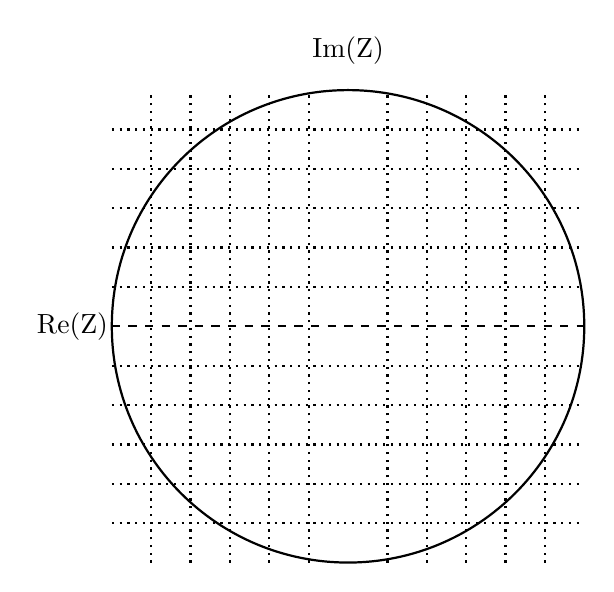
\begin{tikzpicture}
    % Smith chart visualization (very simplified, actual detailed Smith chart would require extensive data)
    \draw[thick] (0,0) circle (3cm);
    \draw[thick, dashed] (-3,0) -- (3,0); % Real axis
    \foreach \x in {-2.5,-2,-1.5,-1,-0.5,0.5,1,1.5,2,2.5} {
        \draw[thick, dotted] (\x,-3) -- (\x,3); % Vertical lines
    }
    \foreach \y in {-2.5,-2,-1.5,-1,-0.5,0.5,1,1.5,2,2.5} {
        \draw[thick, dotted] (-3,\y) -- (3,\y); % Horizontal lines
    }
    \node at (-3.5, 0) {Re(Z)};
    \node at (0, 3.5) {Im(Z)};
\end{tikzpicture}

In conclusion, the Smith chart is specifically designed for calculating and visualizing impedance along transmission lines, making option A the correct choice in this context. Other options, while relevant to RF theory, do not directly relate to the primary function of the Smith chart.
